%
%  Created by Kasper Nybo Hansen on 2011-03-30.
%  Copyright (c) 2011 Kasper Nybo Hansen. All rights reserved.
%
%

\documentclass[10pt]{article}

\RequirePackage{nybohansenPreamble}

\usepackage{fullpage}

\newcommand{\authorName}{Kasper Nybo Hansen}
\newcommand{\authorEmail}{nybo@diku.dk}
\newcommand{\titleName}{Recognition of Traffic Signs \\Exam assignment}
\newcommand{\courseName}{Statistical Methods for Machine Learning}

\author{\authorName \\\texttt{\small{\authorEmail}}}
\title{\textsc{\titleName \\ \courseName}}
% \date{}
\makeindex

\begin{document}

\maketitle 


\section*{Question 1} % (fold)
\label{sec:question_1}
The downloaded dataset contains $26640$ vector samples, where each vector is of dimension $1568 \times 1$. The $26640$ samples is distributed throughout $43$ classes, where each class is a different traffic sign. The samples are HOG features of the observed traffic sign.

Each folder in the downloaded dataset, \texttt{HOG_01}, corresponds to one class. Each file corresponds to one sample. The number of samples, are not equal distributed throughout the classes. I.e. the number of samples taken from each of the $43$ traffic signs are not equal. Figure \ref{fig1} shows the \emph{normalized} histogram of the class frequencies found in the dataset.

\begin{figure}[ht]
\centering
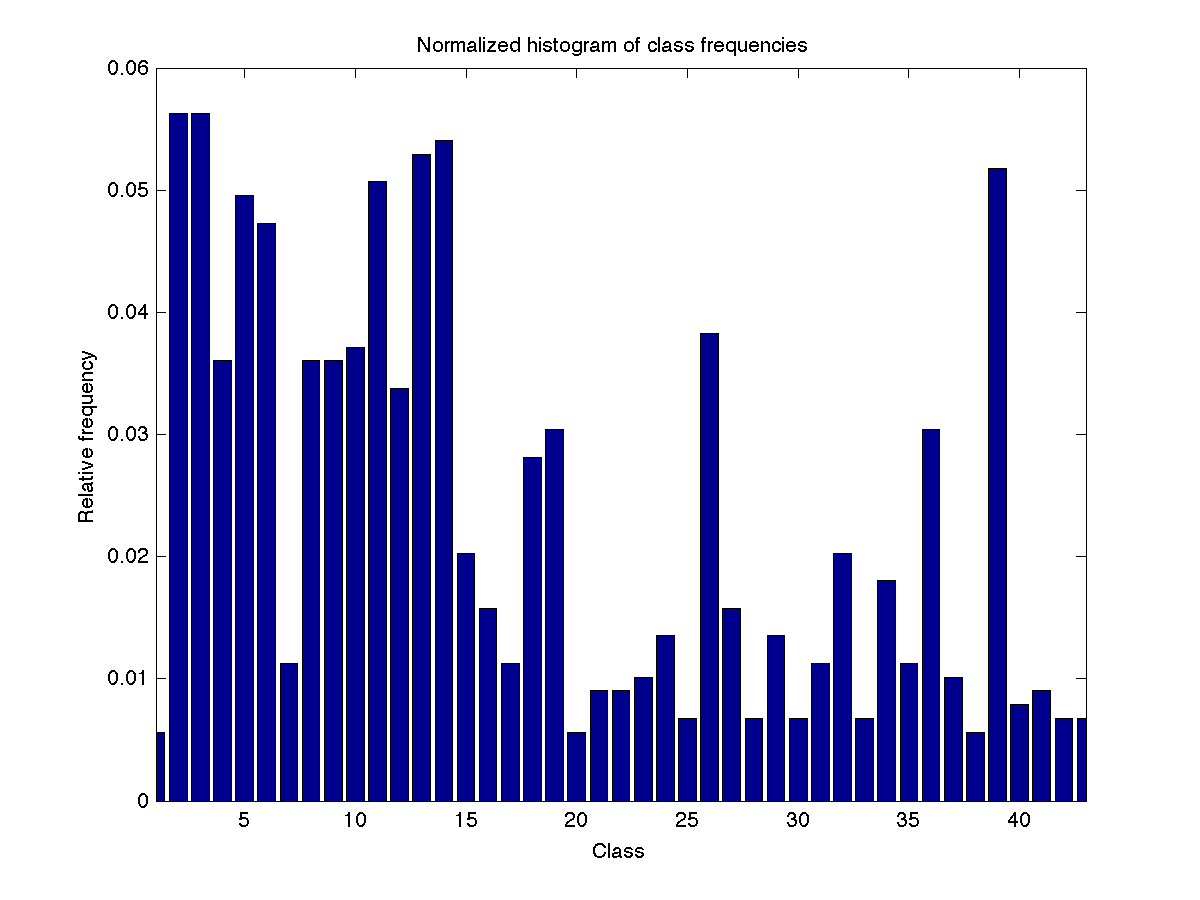
\includegraphics[width=0.65\textwidth]{figures/q1.png}
\caption{Histogram of normalized frequencies of the classes found in the dataset.}
\label{fig1}
\end{figure}


All programming assignments in this exam set is done in MATLAB. The source code to this question can be found in the files \texttt{loadDataSet}, \texttt{initializaDataSet.m} and \texttt{q1.m}. All of the following implementations, assume that \texttt{initializaDataSet.m} has been run.

% section question_1 (end)

\section*{Question 2} % (fold)
\label{sec:question_2}

Principal Component analysis (PCA) can be used for dimensionality reduction, giving the possibility to visualize parts of a high dimensional dataset. The dimensionality reduction is done by finding principal components of a dataset, an projecting the data on to these. It is important to note, that only a part of the variance in the dataset will be present when visualized this way.

I have done PCA on the dataset, $X$, by first centering the dataset i.e
\begin{equation}
  B = X - \bar{X}
\end{equation} 
where $\bar{X}$ is the mean vector of $X$. I then calculate the covariance matrix $C$ of $B$. The eigenvectors of the covariance matrix is the PCA components, and the eigenvalues describes the variation contained in the PCA components. 

I calculate the eigenvalues and eigenvectors of $C$. The eigenvalues are stored as the diagonal elements of a matrix $D$, and the eigenvectors are stored column wise in the matrix $V$. I then sort the eigenvalues in descending order, making sure that the eigenvalues matrix $V$ are sorted the same way. The $i'th$ column in $V$ is now the $i'th$ PCA component. 

The eigenvalues in $D$ contains information about the variation in the corresponding eigenvector in $V$. The total variance is calculated as the sum of all the diagonal elements in $D$. A plot can be made showing the percentage of total variance in the first $k$ components, by calculating the cumulative sum of $D$, and plotting this as a function of the number of components. An example of such a plot, can be seen in figure \ref{fig2}.
  
Figure \ref{fig0} shows a plot of the eigenvalues of the sorted components. Figure \ref{fig2} shows that $90\%$ of the variance is contain within the first $305$ PCA components (This is also confirmed programmatically!).

\begin{figure}[ht]
\centering
\mbox{
    \subfigure[Eigenvalues of the sorted components]{\label{fig0}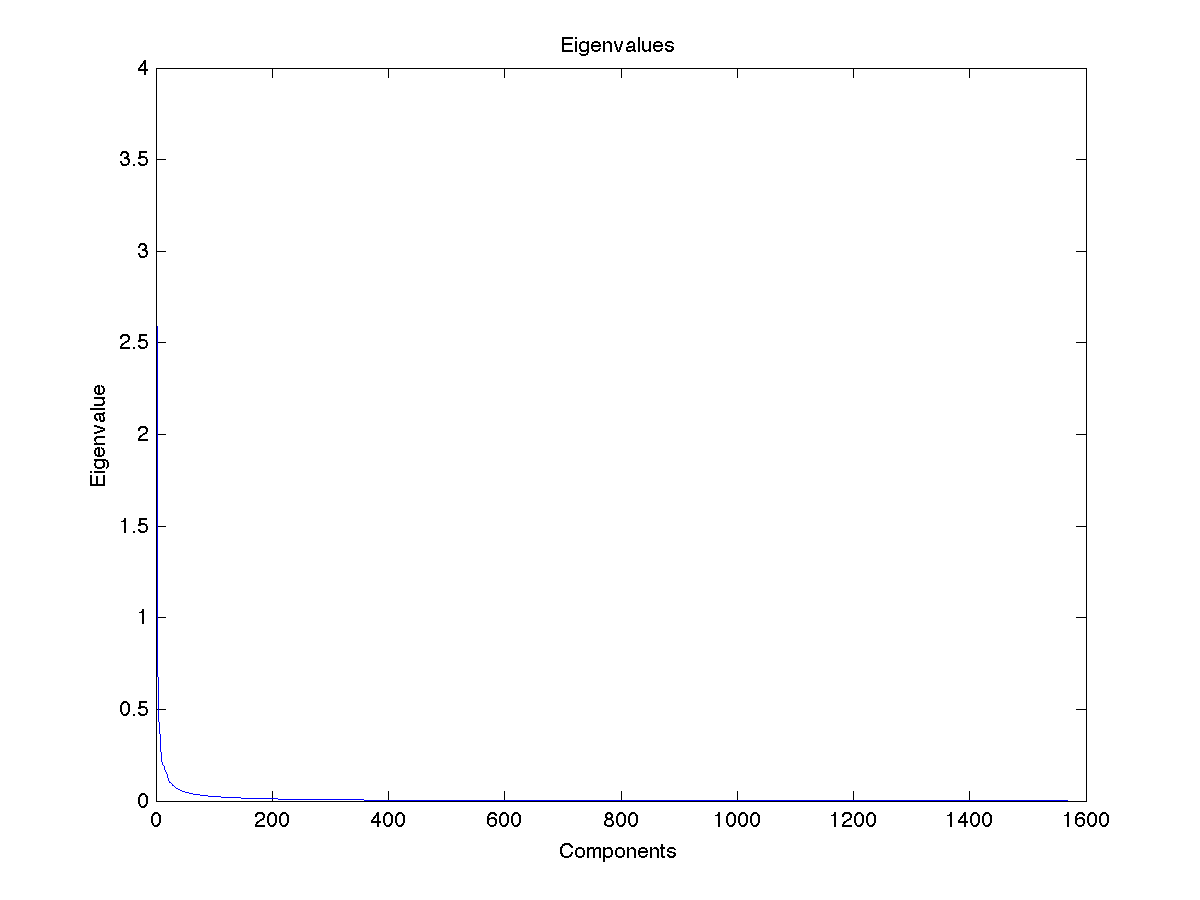
\includegraphics[width=0.5\textwidth]{figures/q2-5.png}} \quad
    \subfigure[$90 \%$ of the variance is contained within the first $305$ principal components.]{\label{fig2}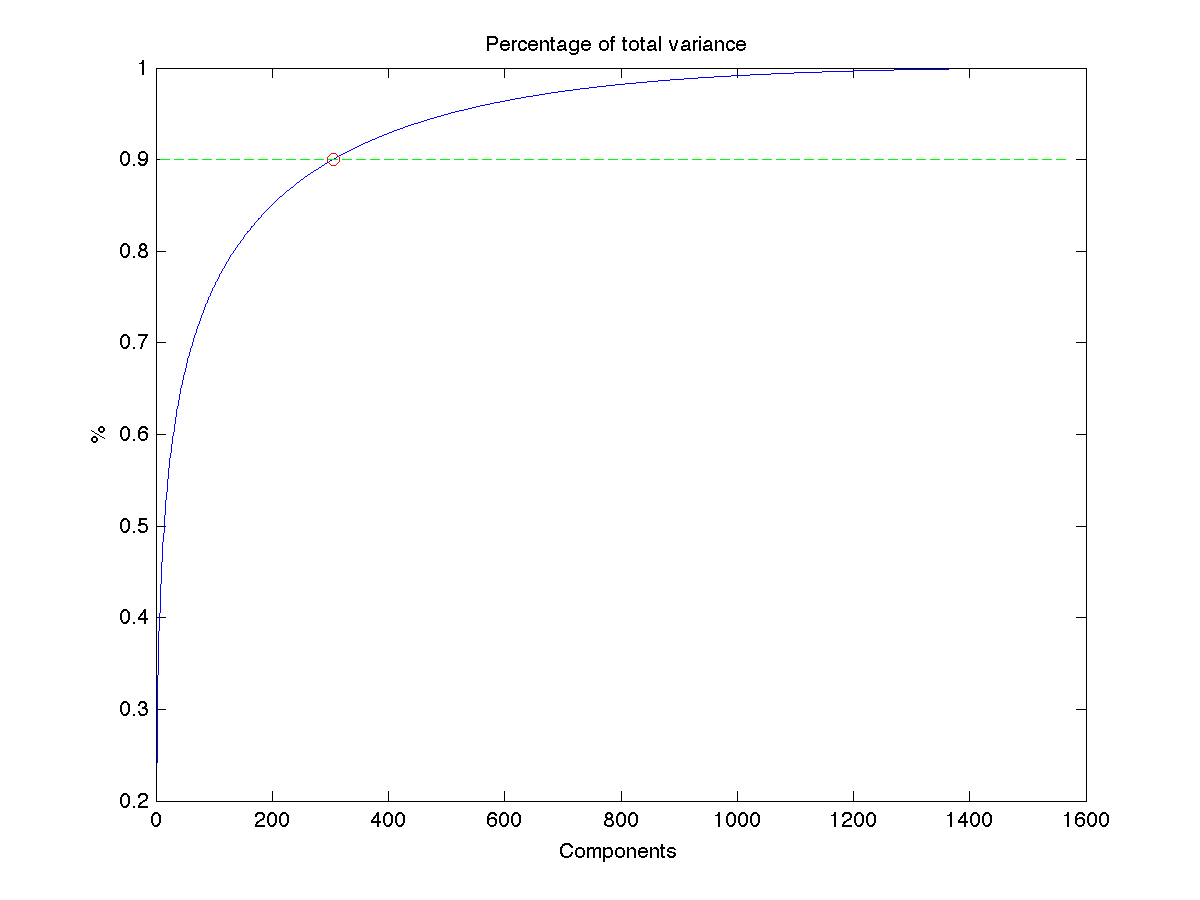
\includegraphics[width=0.5\textwidth]{figures/q2-1.png}}
}                    
\end{figure}
I have projected the dataset on to the first and second PCA components, by multiplying the transposed two principal components on to the centered dataset. I.e.

\begin{equation}
  Y = E^T*B  
\end{equation}
where $E$ is a matrix consisting of two column vectors representing the two PCA components, and $B$ is the centered dataset. The result can be seen on figure \ref{fig3}

\begin{figure}[ht]
\centering
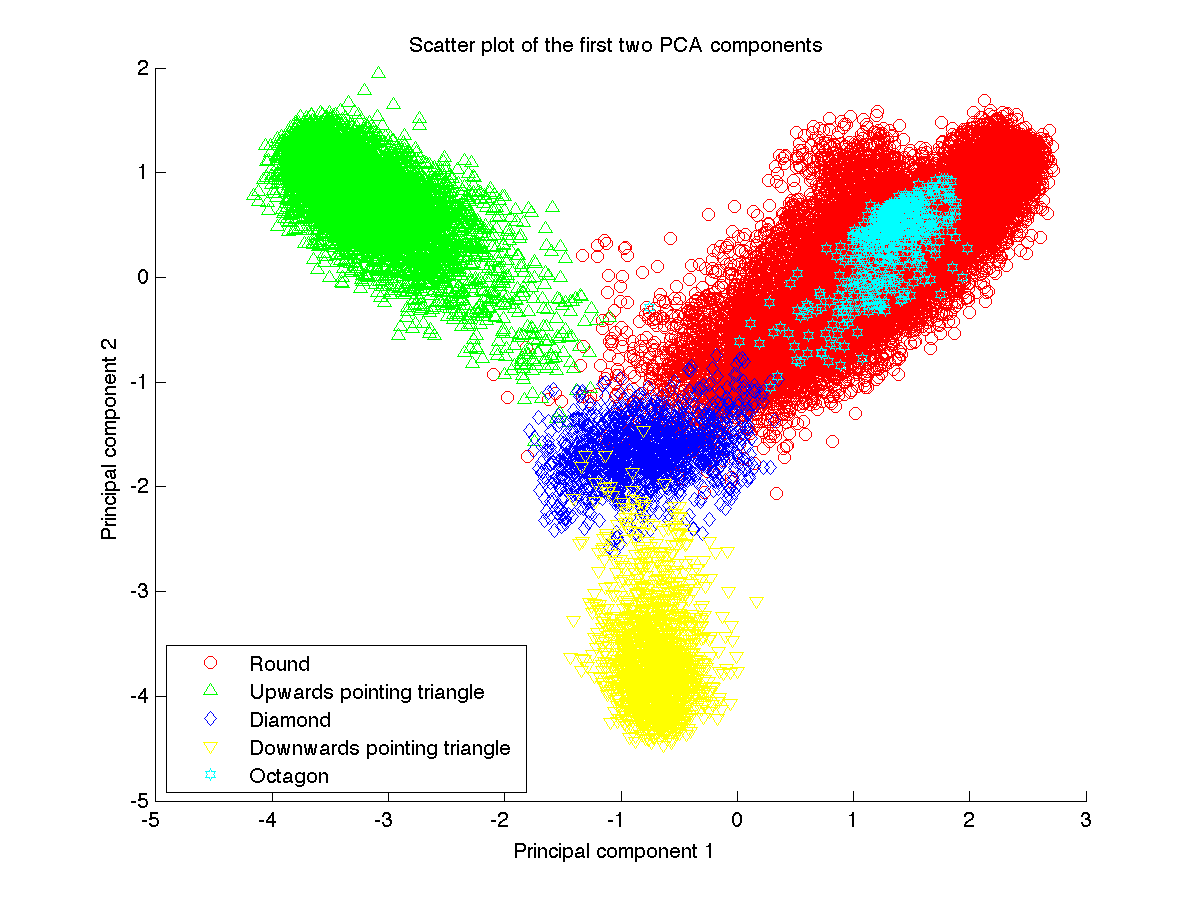
\includegraphics[width=0.9\textwidth]{figures/q2-2.png}
\caption{The dataset projected on to the first two PCA components. Each color/shape represent a different class. There are in total five classes.}
\label{fig3}
\end{figure}

The source code to this question can be found in the file \texttt{q2\_3.m}.
% section question_2 (end)

%\clearpage

\section*{Question 3} % (fold)
\label{sec:question_3}
$K$-means is an unsupervised clustering algorithm. Given $K$ and a dataset, the algorithm partitions the data into $K$ clusters. Unsupervised means that it requires no information about the features present in the dataset.

Let the dataset consists of sample vectors of size $\R^d$. Then the algorithm is initialized by creating $K$ arbitrary centroids all belonging to $\R^d$. Let each centroid has it's own label. 

For each sample vector in the dataset, the distance to all the centroids is calculated. The label of the centroid closest to the datapoint, determines the label of the sample vector. When all sample vectors have been assigned a label, the centroids are recalibrated. 

Recalibration is done by moving each centroid to the mean of the sample vectors having it's label. 

When the recalibration is done, the algorithm restarts and for each sample vector, the distance to the new centroids are calculated. The sample vector is again given the label of the closest centroid.

The algorithm stops when the centroids doesn't move.

For this question I have made my own implementation of the $K$-means algorithm. The source code to this algorithm can be found in the file \texttt{kmeans.m}. 

I have applied my implementation to the dataset from the previous assignment. I applied it with $K=4$. The result can be seen on figure \ref{fig4} and \ref{fig5}. The figure shows the found centroids projected on to the first two PCA components. The algorithm finds the green class nicely, but it is clear that the three other centroids are placed a bit of.

The reason for the misplacement of some of the centroids, is the $K$-means initialization step. The $K$-means algorithm is very sensitive, when it comes to the initial guess of the centroids of the clusters. The difference between figure \ref{fig4} and \ref{fig5} clearly shows this. Figure \ref{fig4} and \ref{fig5} are both made by initializing the algorithm with 4 randomly selected sample vectors as centroids. It is clear that the cluster centroids are placed very differently between the two runs.

\begin{figure}[ht]
\centering
\mbox{
    \subfigure[Random initialization of cluster centroids. Two centroids inside `red/cyan' class, none in `blue' class.]{\label{fig4}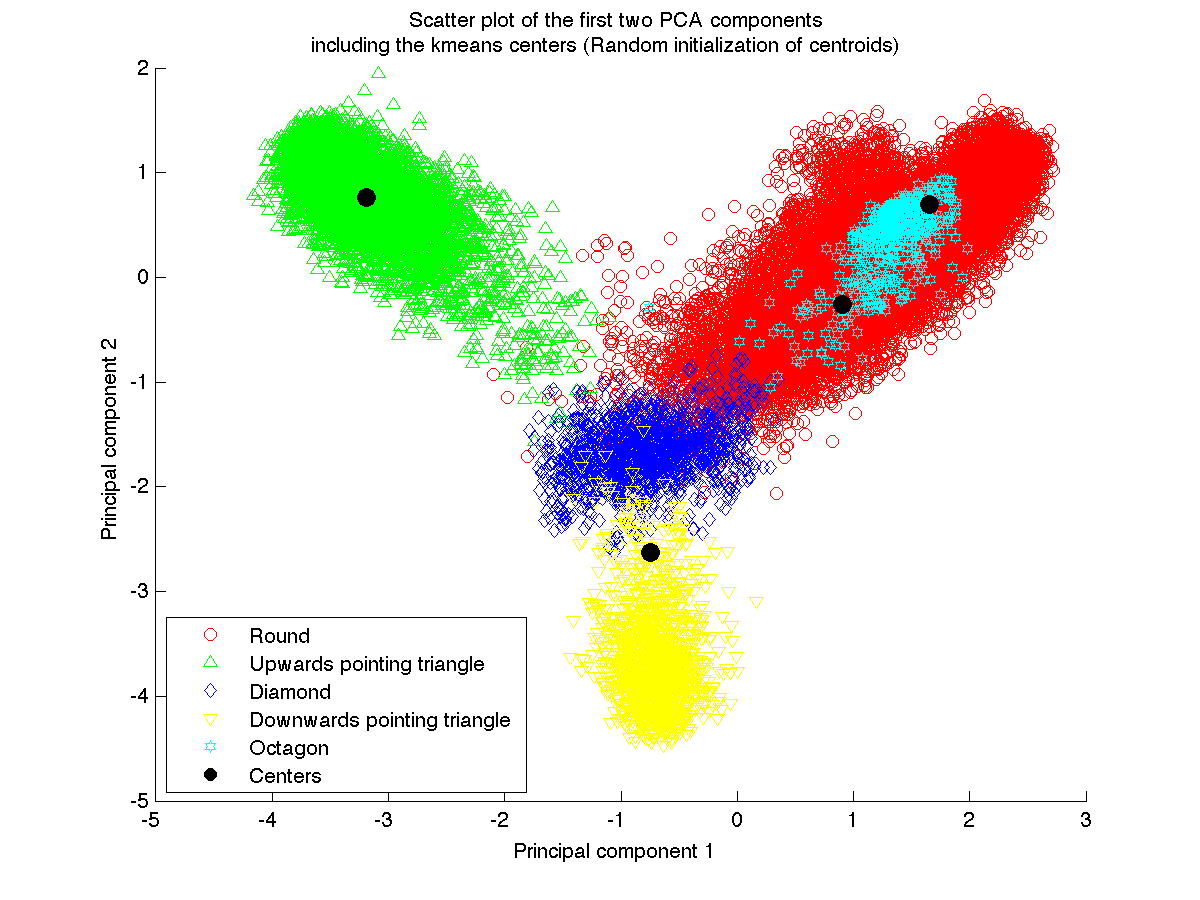
\includegraphics[width=0.5\textwidth]{figures/q2-3.png}} \quad
    \subfigure[Random initialization of cluster centroids. One centroid inside `red/cyan' and one in `blue' class.]{\label{fig5}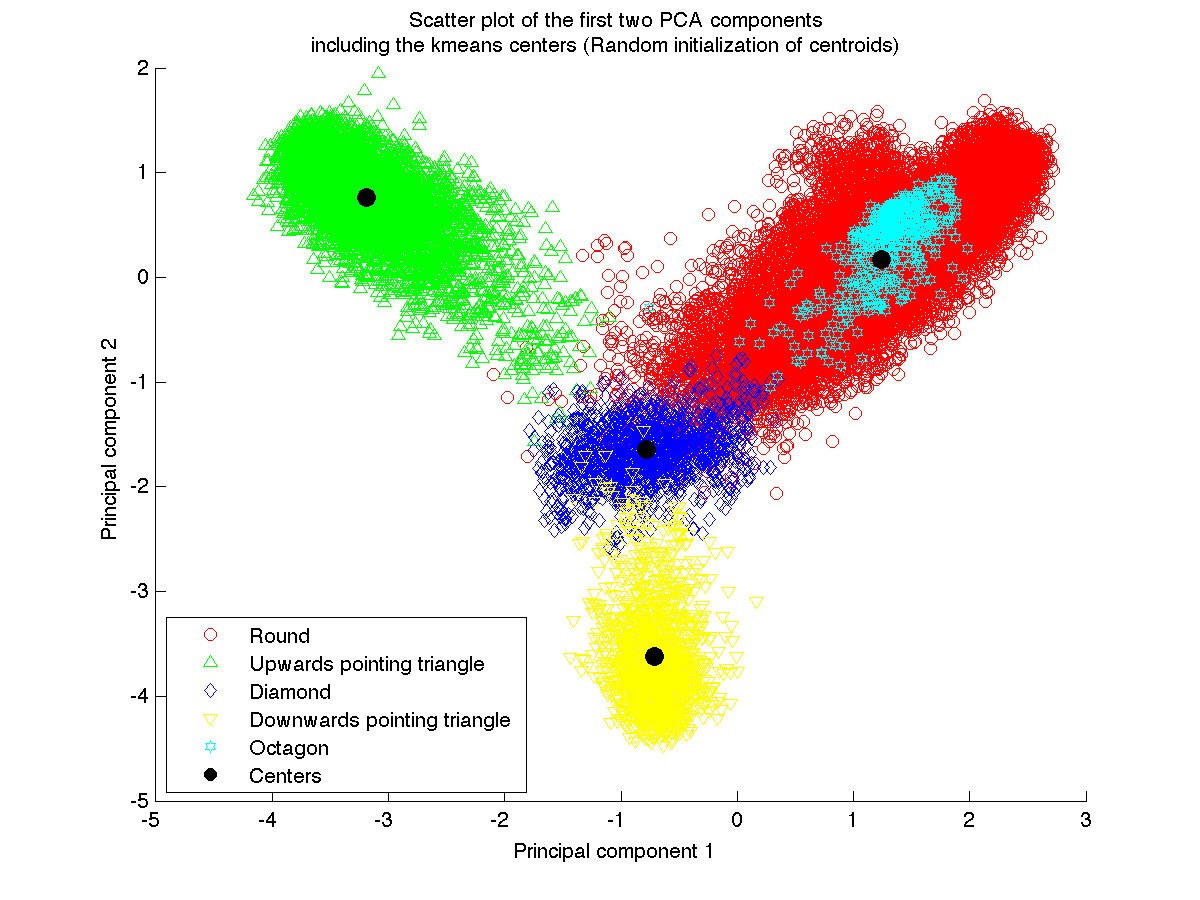
\includegraphics[width=0.5\textwidth]{figures/q2-4.png}}
}                    
\caption{Illustration of the sensitivity in the initialization process. Both figures where made by choosing the cluster centroids randomly from the dataset, but finds completely different centroids.}
\label{label}
\end{figure}

The source code to this question can be found in the file \texttt{q2\_3.m}.
% section question_3 (end)

% \clearpage

\section*{Question 4} % (fold)
\label{sec:question_4}
In this question I will relate the different types of overfitting described in hunch.net\cite{hunch} to this exam set.

\textbf{Traditional overfitting} can occur if we train on to few examples. Luckily for us, we have plenty of data to play around with so this shouldn't be a problem.

\textbf{Parameter tweak overfitting} can occur if we adjust the hyperparameters of the model to perform good on the test set. Parameter tweak overfitting could occur in this assignment, if we didn't make sure that all 30 instances of the same physical sign, is placed in the same subset of the cross validation. If two instances of the same physical signs, where spread across two bins in the cross validation, we would train our model on something that is very `similar' to the test set.

\textbf{Brittle measure} can occur if we instead of $5$-fold cross validation, did $n$-fold cross validation, where $n$ is the number of samples. This type of cross validation is also known as \emph{Leave-one-out cross-validation}.

\textbf{Incomplete Prediction} can occur if we made multiple binary classification models and uses these in the multi-class classification.

\textbf{Data set selection} The following example explains how data set selection can can occur in this assignment. Let the performance of the $k-$NN be very good in one of the folds in the $5$-fold cross validation. We then choose this whole subset as the test set thereby improving the overall results.                                                                                                                                              

\textbf{Choice of measure} can occur if the accuracy calculation is improved when changing the way the accuracy is calculated. In this assignment we are primarily working with classification. This means that the accuracy is based on the misclassifications. I don't see how we can change this accuracy calculation. In the regression assignment, one could use the sum of squares as the error measurement - this would lead to some awkward results possible improving the accuracy.

Since the dataset is almost new\cite{dataURL}, I don't see how the \textbf{Old datasets} method of overfitting can occur. 

Furthermore I don't see how the following methods of overfitting can occur: \textbf{Bad statistics}, \textbf{Human-loop overfitting} and \textbf{reprobleming} in this exam assignment. It is hard to do reprobleming, since the assignment text is very explicit. There is no humans involved in the training nor testing phase, so Human-loop overfitting seems impossible. \\

% section question_4 (end)


                      
The following questions (question 5-8) regards classification. Classification, is the task of labeling a unknown sample from known samples containing labels. It is a supervised learning task, since we use prior knowledge (knowledge of the labels of the training set).


\section*{Question 5} % (fold)
\label{sec:question_5}

In this question I have filtered the training set, such that only the classes 1 and 5 are present. 

\subsection*{Cross-validation} % (fold)
\label{sub:cross_validation}
Each physical traffic sign has $30$ sample vectors present in the dataset. This causes problems, because this can lead to overoptimistic results. Although we are not given the details of the HOG features, it is clear that the $30$ sample vectors taken from the same physical traffic sign is positioned close together in the $1568$ dimensional space. 

This poses a problem, since, unintentionally, we can train on a subset of a physical sign, and test on the other part of the same subset. This would definitely lead to overoptimistic results and should be avoided.

I have partitioned the training data, by randomizing the \emph{physical} signs into $5$ bins. After the randomization, each sign is replaced with it's corresponding $30$ samples. This ensures that the same physical sign is placed in the same cross validation subset.

The cross validation is done as a $5$-fold cross validation. More precisely I have done cross validation in the following way. Let $B$ denote the bin numbers, e.g. $B = \{1,2,3,4,5\}$. Foreach bin $b_i \quad i \in B$ i have used the samples in $b_i$ as test data, and samples in the rest of the bins as training data. Thus each subset of the $5$-fold cross validation acts as a test set once, while acting as part of a training set 4 times.
% subsection cross_validation (end)

\subsection*{Computation of test errors} % (fold)
\label{sub:computation_of_test_errors}
When doing $5$-fold cross validation, the result is 5 intermediate results, a result for each fold. I have used the mean of these 5 intermediate result, as a measurement of how good the classifier is. I have measured the error, as a sum of the number of misclassifications the classifier makes. I.e. foreach classification the classifier makes, I compare the result with the label of the training set, and if the two are different, I consider it as an misclassification.

The accuracy is measured as 
\begin{equation}
  \text{accuracy} = \text{misclassification}/\text{total number of samples}
\end{equation}

% subsection computation_of_test_errors (end)

\subsection*{Linear classification} % (fold)
\label{sub:linear_classification}
I have chosen Linear Discriminant Analysis (LDA) as my linear classification method. I have chosen this method because it gives good result in practice and is highly recommended as a baseline method\cite{LDAslides}. 

In group assignment 2, we made a LDA implementation\cite{assignment2}. I tried solving the classification problem with this implementation, but the performance was very bad. Instead I substituted my own implementation with the MATLAB function \texttt{classify} and the results where very much improved. The result of doing binary classification with MATLAB's LDA implementation can be seen in table \ref{table10}. The table shows the accuracy for each of the $5$-folds cross validation runs, and the mean accuracy. 

As can be seen from the table, the LDA has $\approx 88\%$ accuracy, which must be considered quite good.

\begin{table}
  \begin{center}  
    \begin{tabular}{ | c | c |}
      \hline
      Fold no. & Accuracy\\
      \hline
      1    &     0.87962\\
      2    &     0.88947\\
      3    &     0.89814\\
      4    &     0.89298\\
      5    &     0.86481\\
      \hline
      Mean accuracy &  0.88500\\
      \hline
    \end{tabular}
    \caption{Accuracy over a $5$-fold cross validation when running LDA on the training set.}
    \label{table10}
  \end{center}    
\end{table}   

The source code to this part of the assignment can be found in \texttt{q5\_1.m}.

% subsection linear_classification (end)

\subsection*{Non-linear classification} % (fold)
\label{sub:non_linear_classification}
For the non linear classifier I have chosen to use a Support Vector Machine (SVM) with a Gaussian Radial Basis Function - the same approach as we used in a previous group assignment\cite{assignment3}. I have chosen to use SVM, because it performed well in the group assignment, and is highly recommended by the course responsible.

The gaussian kernel is on the form 
\begin{equation}
  k(x,z) = e^{-\gamma||x-z||^2}
\end{equation}
where $\gamma>0$ is a bandwidth hyperparameter that can be tweaked accordingly. The SVM also has a cost parameter $C$ that can be tweaked. As in the previous group assignment, we can use 
\begin{equation}
  \sigma = \sqrt{1/(2\gamma)}
  \label{eq21}
\end{equation}
instead of $\gamma$. We can then compute $\gamma$ from \ref{eq21} as
\begin{equation}
  \gamma = 1/(2\sigma^2)  
\end{equation} 

Jaakkola's heuristic, provides a reasonable guess of the bandwidth parameter $\sigma$\cite{assignment3}. Let 
\begin{equation}
  G = \{ ||x_i - x_j||\quad | \quad (x_i,y_i),(x_j,y_j) \in S \wedge y_i \neq y_j \}
\end{equation}
for a training set $S$. I.e $G$ is the difference in input space between all pairs in $S$. Jaakkola's heuristic can then be computed as the median of $G$. 

For finding the appropriate SVM hyperparameters I have made a grid search. The grid can be seen in table \ref{table4}.  

\begin{table}
  \begin{center}  
    \begin{tabular}{ | c | c | c | c | c | c | c |}
      \hline
       $i/C$   & 0.1          & 1             & 10           & 100           & 1000          &     10000\\ \hline
       -3 & 0.67331           & 0.87089       & 0.91668      & 0.91853       & 0.91890       &     0.91890\\ \hline
       -1 & 0.81304           & 0.91612       & 0.92606      & 0.92717       & 0.92717       &     0.92717\\ \hline            
       -0 & 0.84555           & 0.92337       & 0.93070      & 0.93070       & 0.93070       &     0.93070\\ \hline      
       1  & 0.86253           & 0.92746       & 0.93389      & 0.93389       & 0.93389       &     0.93389\\ \hline      
       3  & 0.64775           & 0.88994       & 0.89356      & 0.89356       & 0.89356       &     0.89356\\ \hline      
    \end{tabular}
    \caption{Accuracy given different SVM model hyperparameters. The model is most accurate when $i=1$ and $C=10$, yielding an accuracy of $\approx 93\%$}
    \label{table4}
  \end{center}    
\end{table}   
As can be seen from table \ref{table4} the model is most accurate when $i=1$ and $C=10$. The accuracy when running the model with these hyperparameters is $\approx 93\%$. Which is better than the accuracy of the LDA.

The source code to this part of the assignment can be found in \texttt{q5\_2.m} and \texttt{calcSVMModel.m}. Note the implemented code needs the LIBSVM framework\cite{libsvm}. 
% subsection non_linear_classification (end)

% section question_5 (end)

\section*{Question 6} % (fold)
\label{sec:question_6}

For this question, I have chosen to use linear description method (LDA) as my linear classifier and $k$ nearest neighbor ($k-$NN) as my non-linear classification method. In both cases I have used $5$-fold cross validation as described in question 5. Furthermore I have calculated the accuracy of the methods as described in question 5.  

\subsection*{Linear classification} % (fold)
\label{sub:linear_classification2}

For my linear classifier I have chosen to use LDA, again using the MATLAB function \texttt{classify}. The result of running the LDA can be seen in table \ref{table3}. Again the LDA performs quite good, and has an accuracy of $\approx 92\%$. 

\begin{table}
  \begin{center}  
    \begin{tabular}{ | c | c |}
      \hline
      Fold no. & Accuracy\\
      \hline
      1    &     0.91412\\
      2    &     0.93913\\
      3    &     0.93333\\
      4    &     0.92453\\
      5    &     0.92322\\
      \hline
      Average &  0.92686 \\
      \hline
    \end{tabular}
    \caption{Table showing the average accuracy over a $5$-fold cross validation when running LDA on the entire training dataset.}
    \label{table3}
  \end{center}    
\end{table}   




The source code to this question can be found in the file \texttt{q6\_1.m}.

% subsection linear_classification (end)


\subsection*{Non-linear classification} % (fold)
\label{sub:non_linear_classification2}
As my non-linear classification method, I have chosen the basic kernel known as the k nearest neighbor ($k-$NN). K nearest neighbor is a very versatile, yet simple, algorithm that usually performs pretty good regardless of the data it is working on. It is actually in the top 10 data mining algorithms\cite{Wu07doi10.1007/s10115-007-0114-2}.

The algorithm works as follows. The user specifies a $k$ to the algorithm and a data and test set. For each point in the test set, the $k$ nearest neighbors of training set are found. The most frequently label of the $k$ nearest neighbors becomes the label of the test point. This is also the reason why $k-$NN can be slow. It is computational very expensive.

K nearest neighbor is a lazy algorithm. This mean that the algorithm doesn't create a model for the training set. 

$k$ is a parameter that can be tweaked to suit the dataset. In order to find an appropiate $k$ i have done $5$-fold cross validation, on different $k$ values. The result can be seen in table \ref{table2}. Each row in the table corresponds to a $5$-fold cross validation with the $k$ specified in column 1. As can be seen the most accurate result is archieved when $k=20$. The $k$-NN has an accuracy of $71\%$ when $k=20$. This is not as good as the LDA, but still reasonable. 

\begin{table}
  \begin{center}  
    \begin{tabular}{ | c | c |}
      \hline
      $k$ & Average accuracy over $5$-fold cross validation\\
      \hline
        1    &     0.69996\\
        2    &     0.69483\\
        5    &     0.70937\\
       10    &     0.71256\\
       15    &     0.71167\\
       20    &     0.71329\\
       30    &     0.71262\\
       40    &     0.71063\\
       50    &     0.70920\\
      100    &     0.69793\\
      250    &     0.66310\\        
      \hline
    \end{tabular}
    \caption{Average accuracy over a $5$-fold cross validation when running $k-$NN with different $k$'s. As can be seen, $k=20$ yields the best accuracy.}
    \label{table2}
  \end{center}    
\end{table}   

I have implemented the $k-$NN algorithm in the file \texttt{kNN.m}. Other source code files related to this question includes \texttt{knnHelper.m} and \texttt{q6_2.m}.

% subsection non_linear_classification (end)

% section question_6 (end)

\section*{Question 7} % (fold)
\label{sec:question_7}
I have tested the previous implemented classifiers on the supplied test set. For each classifier implemented in the previous assignments, I have chosen the best performing model. I have then used this model to classify the traffic signs in the test set.

The following sub sections elaborate on the results.

\subsection*{Testing binary classification using LDA} % (fold)
\label{sub:binary_classification}
In the training phase, the $5$-fold cross validation yielded a mean accuracy of $0.88500$. I have testet the implementation on the test set by using the whole training set as training, and the test set as test. The result is a average accuracy of $0.92196$. The classifier actually performs $3.596\%$ better on the test set than the training set. 

The source code to this question can be found in \texttt{q7\_1.m}.

% subsection binary_classification (end)

\subsection*{Testing binary classification using SVM} % (fold)
\label{ssub:testing_binary_classification_using_svm}
In question 5 I found that the SVM model performed best with hyperparameters, $i=1$ and $C=10$. I have therefore used these hyperparameters in the testing phase. Running the SVM with these chosen hyperparameters and the whole training set as training data, and the test set as test data I get an accuracy of $0.93389$. Compared to the mean accuracy off the $5$-fold cross validation done in the training phase, this is $4.35\%$ better.

The source code to this question can be found in \texttt{q7\_2.m}.
% subsubsection testing_binary_classification_using_svm (end)

\subsection*{Testing multi-class classification with LDA} % (fold)
\label{sub:multi_class_classification}

The accuracy of the multi-class LDA classifier done in question 6, was $0.92686$. When I run the LDA classifier with the whole training set as training data, and the whole test set as test data, I get an accuracy of $0.94510$. The classifier is thus $1.824\%$ more accurate on the test set.

The source code to this question can be found in \texttt{q7\_3.m}.

% subsection multi_class_classification (end)

\subsection*{Testing multi-class classification using $k-$NN} % (fold)
\label{sub:testing_multi_class_classification_using_knn}
As the non linear method, i made use of $k-$NN in question 6, when doing multi-class classification. From Question 6, I have that the $k-$NN performed best when $k=20$. I have therefore chosen to set $k=20$ when classifying the test set. 

Again the whole training set is used as training, and the whole test set is used as test data. The result of classifying the test set, is an accuracy of $0.76776$, which is $5.447\%$ better than the average of the $5$-folds cross validation.  

The source code to this question can be found in \texttt{q7\_4.m}.
% subsection testing_multi_class_classification_using_knn (end)

\subsection*{Overall performance} % (fold)
\label{sub:overall_performance}

All of the implementations performed better on the testing data, than the training data. One possible explanation for this behavior could be, that we use the whole test set as the testing data, thereby dramatically increasing the number of training points.

It comes to no surprise that the LDA implementations archives a high degree of accuracy. Looking at the results page of the \emph{The German Traffic Sign Recognition Benchmark}\cite{resultsURL} the combination of LDA and the \texttt{HOG01} dataset is scoring high.

What comes as a surprise, is how good the $k-$NN implementation performs, compared to how simple it is. Even in the multi-class classification the $k-$NN archives an accuracy of $76\%$.
% subsection overall_performance (end)

% section question_7 (end)

\section*{Question 8} % (fold)
\label{sec:question_8}

I have used linear regression to solve the binary classification and multi-class classification problem. In both cases i have used $5$-fold cross validation on the training set, and partitioned the data as explained in question 5. Furthermore I have calculated the accuracy as explained in question 5. I have done this so I can compare the results with the one from question 5 and 6.

I have constructed the design matrix as defined in Bishop\cite{Bishop:2006:PRM:1162264} 3.16. Each row of the design matrix is a sample vector. The \emph{Moore-Penrose pseudo inverse} of the design matrix is calculated, and the maximum likelihood is calculated as defined in Bishop 3.15. Finally the model is applied to the training set as defined in 3.3 of Bishop. 

The \emph{Moore-Penrose pseudo inverse} is computational expensive to calculate. In order to speed things up, I have used a alternative implementation taken from\cite{DBLP:journals/corr/abs-0804-4809}. The optimized Moore-Penrose pseudo inverse function can be found in the file \texttt{geninv.m}.

The result can be seen in table \ref{table1}.

\begin{table}
  \begin{center}  
    \begin{tabular}{ | c | c | c |}
      \hline
      Fold no. & Accuracy binary case & Accuracy multi-class case\\
      \hline
      1       &  0.87962  &  0.13032\\
      2       &  0.83157  &  0.10244\\
      3       &  0.91666  &  0.10168\\
      4       &  0.88421  &  0.10468\\
      5       &  0.92592  &  0.12209\\
      \hline
      Average &  0.88760  &  0.11224\\
      \hline      
    \end{tabular}
    \caption{Performance of using linear regression to do binary and multi-class classification. In average the classifier is correct in $\approx 88\%$ of the cases when doing binary classification, and $\approx 11\%$ when doing multi-class classification.}
    \label{table1}
  \end{center}    
\end{table}   
                                       
Compared to the result from question 5 (Binary case), the abuse of regression for doing classification, actually performs pretty well. In average the regression method is $0.88760$ accurate, whereas the best binary classifier, SVM, was $0.93389$ accurate. This means that the SVM is only $4.269\%$ better, compared to the regression method.

If we compare the regression method with the LDA implementation from the binary case, then the LDA is only $3.925\%$ better.

As can be seen from table \ref{table1}, the regression method fails miserably when used on the multi-class classification case. The best multi-class classifier from question 6 was LDA. LDA archived an accuracy of 0.92686. This is $81.462\%$ better than the regression method.
                                                                                                                    
The source code to this question can be found in the files \texttt{regression.m}, \texttt{q8\_1.m} and \texttt{q8\_2.m}. 

% section question_9 (end)

\section*{Question 9} % (fold)
\label{sec:question_9}

We know that $1$ out of $10^5$ ROIs is a traffic sign. Let $P(A)$ define the probability of observing a traffic sign, then $P(A) = 10^{-5}$. Let $P(!A)$ define the probability of not observing a traffic sign, then $P(!A) = 1-10^{-5}$. Let $P(B)$ define the probability that the classifier classifies the ROI as belonging to the positive class. Let $P(!B)$ be the probability that the classifier classifies the ROI as belonging to the negative class. 

It is stated that the probability, that the classifier classifies a positive class as positive is $99\%$\cite{assignment}. Thus $P(B|A)=0.99$ and $P(!B|A)=0.01$. 

Furthermore it is stated that the probability, that the classifier classifies a negative class as negative, is $99\%$\cite{assignment}. Thus $P(!B|!A) = 0.99$ and $P(B|!A) = 0.01$.

The probability of a observing a sign, $P(B)$, can then be calculated as the sum  
\begin{equation}
  P(B) = P(B|A)P(A)+P(B|!A)P(!A) = 0.99 \cdot 10^{-5} + 0.01 \cdot (1-10^{-5}) = 0.0100098
\end{equation} 

With $10^6$ ROI's this yields that $1.00098\%$ would be classified as a sign corresponding to $\approx 10010$ ROI's classified as positive. 

Bayes' theorem states
\begin{equation}
  P(A|B) = \frac{P(B | A) P(A)}{P(B)}
  \label{bayes}
\end{equation}

The probability of a false positive, $P(!A|B)$, can be calculated by (\ref{bayes}) 
\begin{equation}
P(!A|B) = \frac{P(B|!A)P(!A)}{P(B)} = \frac{0.01 \cdot (1-10^{-5})}{0.0100098} = 0.999010969    
\end{equation}
So given $10010$ ROIs classified as positive, the expectation is that $99.9010969\%$ is false positives. This corresponds to $\approx 10000$. Note that I have rounded the numbers, since fractions of a ROI doesn't make sense in this scenario.

% section question_9 (end)

\bibliographystyle{abbrv}
\bibliography{bibliography}

\end{document}